\documentclass[t,table,usenames,dvipsnames]{beamer}

\usetheme{CambridgeUS}
\usecolortheme{beaver}
\setbeamertemplate{navigation symbols}{}

\usepackage[utf8]{inputenc}
\usepackage[croatian]{babel}

\usepackage{datetime}
\renewcommand{\dateseparator}{.}
\newcommand{\todayiso}{\twodigit\day \dateseparator \twodigit\month \dateseparator \the \year}
\date{\todayiso}

\usepackage{listing}
\usepackage{graphicx}
\usepackage{subcaption}
\usepackage{multirow}
\usepackage{color}
\definecolor{LightGray}{gray}{0.9}
\captionsetup{compatibility=false}

\title[NKOSL]{Napredno korištenje operacijskog sustava Linux}
\author[Dominik Barbarić]{Dominik Barbarić\\{\small Nositelj: doc.dr.sc. Stjepan Groš}}
\subtitle{3. Mreže}
\institute[FER]{Sveučilište u Zagrebu\\Fakultet elektrotehnike i računarstva}

\begin{document}

{
	\setbeamertemplate{footline}{}
	\begin{frame}
		\maketitle
	\end{frame}
}

\begin{frame}
	\frametitle{Sadržaj}
	\tableofcontents
\end{frame}

\section{TCP/IP}

\begin{frame}
	\frametitle{Modeli mreža}
	\framesubtitle{Prisjetimo se...}
	\centering
	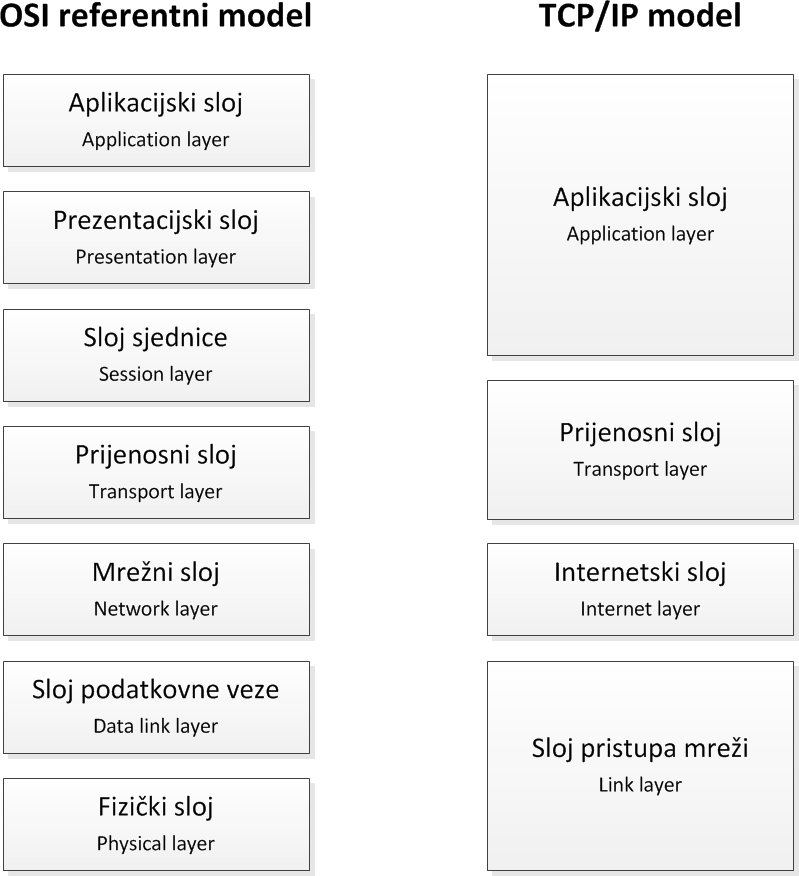
\includegraphics[width=0.5\textwidth]{osi_tcpip.png}
\end{frame}

\begin{frame}
	\frametitle{Modeli mreža}
	\framesubtitle{Prisjetimo se...}
	\begin{itemize}
		\item TCP/IP je najraširenija implementacija OSI modela
		\item Komutacija paketa
		\item IP omogućuje globalnu komutaciju
	\end{itemize}
	\vfill
	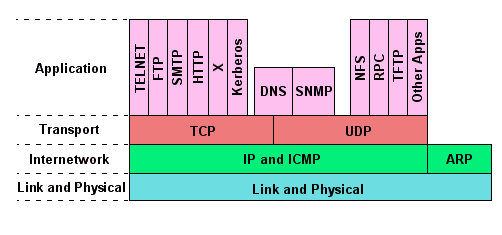
\includegraphics[width=0.8\textwidth]{service_layer.png}
\end{frame}

\begin{frame}
	\frametitle{Adresiranje u TCP/IP modelu}
	\textbf{Sloj pristupa mreži}
	\begin{itemize}
		\item Različito implementiran za svaku metodu pristupa (Ethernet, WLAN, ADSL, DOCSIS, \dots)
	\end{itemize}
	\vfill
	\begin{itemize}
		\item \textbf{MAC (Media Access Control)}
		\begin{itemize}
			\item Odgovara drugom sloju (\textit{Layer 2}) OSI modela
			\item Osigurava pristup mediju, tj. dijelu mreže s kojom je uređaj izravno povezan
			\item Svaki mrežni uređaj ima jedinstvenu (hardversku) \emph{MAC adresu} oblika
			\item[] \texttt{0a:1b:2c:3d:4e:5f} \hfill (48b u hex zapisu) \hfill \,
		\end{itemize}
		\item MAC protokol omogućuje komunikaciju između izravno povezanih uređaja
	\end{itemize}
\end{frame}

\begin{frame}
	\frametitle{Adresiranje u TCP/IP modelu}
	\textbf{Internetski sloj}
	\begin{itemize}
		\item Odgovara trećem sloju (\textit{Layer 3}) OSI modela
		\item Omogućuje komutaciju između Layer 2 mreža
		\item Adresiranje \emph{IPv4 i IPv6 adresama} oblika
		\item[] \texttt{192.168.100.100} \hfill (IPv4 - 32b u dec zapisu)
		\item[] \texttt{fc00:0000:0000:0000:0000:0000:0001:00db}
		\item[] \texttt{fc00::1:db}
		\item[] \hfill (IPv6 -128b u potpunom i skraćenom zapisu)
	\end{itemize}
\end{frame}

\begin{frame}
	\frametitle{Adresiranje u TCP/IP modelu}
	\textbf{IPv4}
	\begin{itemize}
		\item ARPANET 1983.
		\item Adrese se sastoje od 4 okteta = 32 bita
		\item Ukupno adresabilno
		\item[] $2^{32} = 4,294,967,296$ adresa
	\end{itemize}
	\vfill
	\textbf{IPv6}
	\begin{itemize}
		\item Adrese se sastoje od 8 grupa od 16 bita = 128 bita
		\item Prikaz heksadekadskim znamenkama
		\item Ukupno adresabilno
		\item[] $2^{128} = 3.403 \cdot 10^{38}$ adresa
	\end{itemize}
\end{frame}


\begin{frame}
	\frametitle{Adresiranje u TCP/IP modelu}
	\textbf{Subnet}
	\begin{itemize}
		\item Dio mreže s vlastitim rasponom IP adresa koji nema izravnu vezu s drugim takvim dijelom mreže
		\item Subnet je definiran IP adresom mreže i \textit{subnet maskom}
	\end{itemize}
\end{frame}

\begin{frame}[fragile]
	\frametitle{Adresiranje u TCP/IP modelu}
	\framesubtitle{Primjer određivanja subneta}
	\footnotesize
	Mreža je određena adresom mreže i subnet maskom
	\begin{verbatim}
Network: 172.16.64.0
Mask:    255.255.192.0
	\end{verbatim}
	Subnet mask se raspisom u binarni oblik može zapisati:
	\begin{verbatim}
         11111111.11111111.11000000.00000000
	\end{verbatim}
	Na isti način adresa mreže se može zapisati:
	\begin{verbatim}
         10101100.00010000.01000000.00000000
	\end{verbatim}
	Dvije IP adrese pripadaju istom subnetu ako su im svi bitovi na mjestima gdje se u maski nalazi \texttt{1} isti. Zadana mreža obuhvaća sve IP adrese oblika:
	\begin{verbatim}
         10101100.00010000.01******.********
	\end{verbatim}
	U decimalnom zapisu:
	\begin{verbatim}
         172.16.64.0 - 172.16.127.255
	\end{verbatim}
\end{frame}

\begin{frame}[fragile]
	\frametitle{Adresiranje u TCP/IP modelu}
	\begin{verbatim}
	Network: 172.16.64.0
	Mask:    255.255.192.0
	\end{verbatim}
	\begin{itemize}
		\item \textbf{Uočiti} - U svakoj subnet maski jedinice se nužno nalaze na višim bitovima, a nule na nižim
		\item Nemoguća je maska u kojoj se \texttt{0} nalazi između dvije \texttt{1}
	\end{itemize}
	\begin{itemize}
		\item \textbf{CIDR notacijom} adresa mreže se zapisuje u obliku
		\item[] \texttt{172.16.64.0/18}
		\item Broj iza adrese mreže (\texttt{/18}) odgovara broju jedinica u subnet maski
	\end{itemize}
\end{frame}

\begin{frame}
	\frametitle{Adresiranje u TCP/IP modelu}
	\framesubtitle{Posebni rasponi i adrese}
	\begin{minipage}[t]{0.45\linewidth}
	\textbf{Lokalne mreže}
	\begin{itemize}
		{\ttfamily
			\item[] 10.0.0.0/8
			\item[] 172.16.0.0/12
			\item[] 192.168.0.0/16
			\item[] fc00::/7
		}
	\end{itemize}
	\end{minipage}
	\begin{minipage}[t]{0.45\linewidth}
	\textbf{Link-local mreže}
	\begin{itemize}
		{\ttfamily
			\item[] 169.254.0.0/16
			\item[] fe80::/10
		}
	\end{itemize}
	\end{minipage}
	\vfill 
	\textbf{Multicast adrese}
	\begin{itemize}
		{\ttfamily 
			\item[] 224.0.0.0/4
		}
	\end{itemize}
	\textbf{Loopback adresa}
	\begin{itemize}
		{\ttfamily
			\item[] 127.0.0.1
			\item[] ::1
		}
	\end{itemize}
\end{frame}

\begin{frame}
	\frametitle{Adresiranje u TCP/IP modelu}
	\framesubtitle{Posebni rasponi i adrese}
	\begin{itemize}
		\item Unutar raspona subneta postoje dvije posebne adrese
		\item Računala na mreži \textbf{ne mogu} zauzeti navedene adrese
	\end{itemize}
	\vfill
	\textbf{Adresa mreže}
	\begin{itemize}
		\item Prva adresa u rasponu
		\item Primjer
		\item[] \texttt{192.168.20.0}
	\end{itemize}
	\textbf{Broadcast adresa}
	\begin{itemize}
		\item Posljednja adresa u rasponu
		\item Primjer
		\item[] \texttt{192.168.20.255}
	\end{itemize}
	{\small Primjeri su dani za subnet s rasponom 192.168.20.0/24}
\end{frame}

\subsection{IP konfiguracija}

\begin{frame}
	\frametitle{IP konfiguracija}
	IP adresa se dodjeljuje
	\begin{itemize}
		\item Dinamički - DHCP protokol
		\item Statički
	\end{itemize}
	\vspace{1em}
	Konfiguracija se obavlja kroz
	\begin{itemize}
		\item networking
		\item netctl
		\item systemd-networkd
	\end{itemize}
	\begin{itemize}
		\item NetworkManager
		\item wicd
	\end{itemize}
\end{frame}

\begin{frame}[fragile]
	\frametitle{IP konfiguracija}
	\framesubtitle{\texttt{/etc/network/interfaces}}
	\vspace{-1em}
	\begin{verbatim}
auto eth0
iface eth0 inet static
    address 192.168.1.5
    netmask 255.255.255.0
    gateway 192.168.1.254

auto eth1
iface eth1 inet dhcp
	\end{verbatim}
	\begin{itemize}
		\item \texttt{auto eth0} - \texttt{eth0} se omogućuje pri startupu
		\item \texttt{iface eth0 inet static} - \texttt{eth0} ima dodijeljenu statičku IP adresu
		\item \texttt{iface eth1 inet dhcp} - \texttt{eth1} traži dinamičku IP adresu
	\end{itemize}
\end{frame}

\begin{frame}
	\frametitle{IP konfiguracija}
	\begin{itemize}
		\item \texttt{/etc/network/interfaces} se čita prilikom uključivanja i isključivanja mrežnog adaptera
		\item[] \texttt{ifup eth0} \hspace{2em} \texttt{ifdown eth0}
	\end{itemize}
	\begin{itemize}
		\item Neke naredbe za promjenu konfiguracije
	\end{itemize}
	\begin{table}[h]
		\rowcolors{1}{White}{LightGray}
		\begin{tabular}{p{4cm} p{3cm} p{3cm}}
			\rowcolor{BlueViolet!20}Operacija & \texttt{ifconfig} & \texttt{ip} \\
			Pregled konfiguracije & \texttt{ifconfig} & \texttt{ip addr show} \\ & & \texttt{ip link show} \\
			Uključenje i isključenje sučelja & \texttt{ifconfig <interface> up|down} & \texttt{ip link set <interface> up|down} \\
			Podešavanje IP adrese & \texttt{ifconfig <interface> <IP>} & \texttt{ip address add|del <IP> dev <interface>}
		\end{tabular}
	\end{table}
\end{frame}

\subsection{Routing}
\begin{frame}[fragile]
	\frametitle{Routing}
	\begin{itemize}
		\item Povezivanje subneta ostvaruje se \emph{routing}om
		\item Računalo ima konfigurirane rute preko kojih ostvaruje povezanost sa drugim mrežama
	\end{itemize}
	\begin{itemize}
		\item Rute su određene odredišnom adresom i adresom routera ili gatewaya
	\end{itemize}
	{\footnotesize \begin{verbatim}
# route -n
Kernel IP routing table
Destination   Gateway       Genmask        Flags Metric Ref  Use Iface
192.168.1.0   0.0.0.0       255.255.255.0  U     0      0      0 eth0
10.0.0.0      192.168.1.2   255.0.0.0      UG    1      0      0 eth0
0.0.0.0       192.168.1.10  0.0.0.0        UG    0      0      0 eth0

# ip route show
192.168.99.0/24 dev eth0  scope link
10.0.0.0/8 via 192.168.1.2  scope link  dev eth0  metric 1
default via 192.168.1.10 dev eth0
	\end{verbatim} }
\end{frame}

\subsection{DNS}
\begin{frame}[fragile]
	\frametitle{DNS}
	\begin{itemize}
		\item Prevođenje imena računala (tekstualne adrese) u IP adresu
		\item DNS server
		\item IP adresu servera klijenti dobivaju
		\begin{itemize}
			\item Putem DHCP-a
			\item Ručnom konfiguracijom
			\item[] \texttt{/etc/resolv.conf}
			\item[] Uređivanje pomoću spomenutih alata
		\end{itemize}
	\end{itemize}
	\begin{verbatim}
	nameserver 8.8.8.8
	nameserver 8.8.4.4
	\end{verbatim}
\end{frame}

\begin{frame}[fragile]
	\frametitle{DNS}
	DNS server - \texttt{bind}
	\begin{itemize}
		\item Svaka domena (npr. \texttt{fer.hr}) ima svoj \textit{authority}
		\item[] \verb|$ dig soa fer.hr|
		\item Primary i secondary DNS server
		\item[] \verb|$ dig ns fer.hr|
	\end{itemize}
	\begin{itemize}
		\item Svi zapisi o nekoj domeni (\textit{records}) nalaze se u \textit{zone fileu}
		\item Proučiti bind konfiguraciju
	\end{itemize}
	\begin{verbatim}
    $ dig www.fer.hr
    www.fer.hr.    3600   IN   A   161.53.72.119
	\end{verbatim}
\end{frame}

\begin{frame}[fragile]
	\frametitle{DNS}
	Reverse DNS lookup
	\begin{itemize}
		\item Prevođenje IP adresa u domain nazive
		\item Posebne zone s PTR recordima
	\end{itemize}
	\begin{verbatim}
$ dig -x 161.53.72.119
119.72.53.161.in-addr.arpa. 86400 IN	PTR	skynet.cc.fer.hr.
	\end{verbatim}
\end{frame}

\subsection{iptables}
\begin{frame}
	\frametitle{iptables}
	\textbf{iptables}
	\begin{itemize}
		\item Firewall na Linuxu
		\item \emph{Netfilter} framework u kernelu
	\end{itemize}
	
	\begin{itemize}
		\item Provjerava, mijenja, prosljeđuje ili odbacuje pakete prema pravilima u tablici
		\item Tablica se sastoji od lanaca (\emph{chains}), a lanci od pravila (\emph{rules})
		\item Svako pravilo je definirano oblikom paketa na koji se odnosi i akcijom koju obavlja nad tim paketom (\emph{target})
	\end{itemize}
\end{frame}

\begin{frame}
	\frametitle{iptables}
	\centering
	\vspace{-1em}
	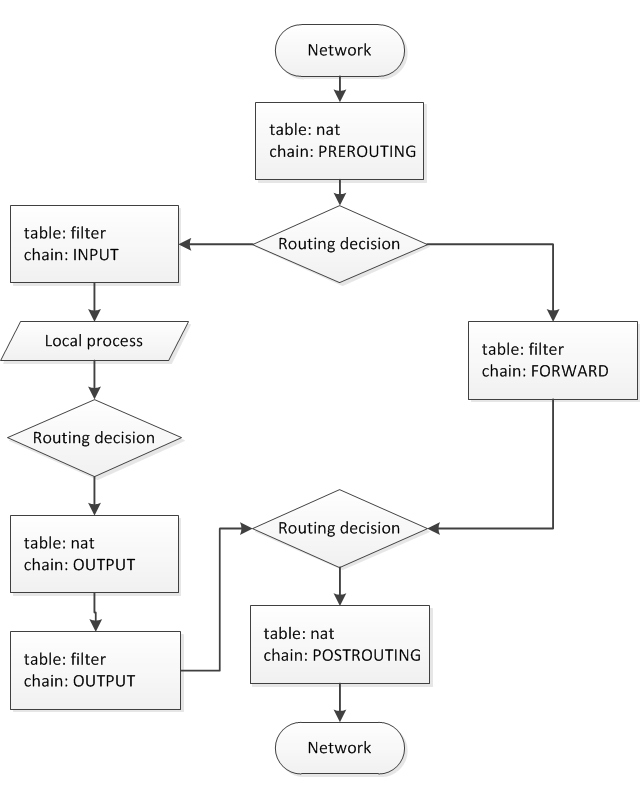
\includegraphics[width=0.5\textwidth]{iptables.png}
\end{frame}

\begin{frame}
	\frametitle{Network address translation (NAT)}
	\begin{itemize}
		\item Za povezivanje lokalnih mreža koristi se prevođenje adresa
		\item Sva računala koja koriste NAT kao routu prema nekoj drugoj mreži dobivaju \textit{istu IP adresu} na odredišnoj mreži
		\item Implementirano u \texttt{iptables}
	\end{itemize}
	\vfill
	Razlikovati
	\begin{itemize}
		\item \textbf{SNAT} (Source NAT)
		\item[] Postupak prevođenja adrese odlaznim paketima
		\item \textbf{DNAT} (Destination NAT)
		\item[] Postupak prevođenja adrese dolaznim paketima
	\end{itemize}
\end{frame}

\begin{frame}[fragile]
	\frametitle{Network address translation (NAT)}
	\small
	\begin{block}{NAT za sve pakete od \texttt{eth1} na \texttt{eth0}}
	\begin{verbatim}
# iptables -t nat -A POSTROUTING -o eth0 -j MASQUERADE
# iptables -A FORWARD -i eth0 -o eth1 -m state
--state RELATED,ESTABLISHED -j ACCEPT
# iptables -A FORWARD -i eth1 -o eth0 -j ACCEPT
	\end{verbatim}
	\end{block}
	\begin{block}{DNAT za HTTP server na internoj adresi 192.168.20.20}
	\begin{verbatim}
# iptables -t nat -A PREROUTING -p tcp -d 161.53.66.200 
     --dport 80 -j DNAT --to-destination 192.168.20.20
	\end{verbatim}
	\end{block}
	\begin{block}{NAT 1:1}
	\begin{verbatim}
# iptables -t nat -A PREROUTING -d 161.53.66.202 -j DNAT 
     --to-destination 192.168.20.30
# iptables -t nat -A POSTROUTING -s 192.168.20.30 -j SNAT
     --to-destination 161.53.66.202
	\end{verbatim}
	\end{block}
\end{frame}

\begin{frame}[fragile]
	\frametitle{Dodatne IP adrese}
	\begin{itemize}
		\item Jedan mrežni adapter može imati više IP adresa
		\item Linux svaku adresu tretira kao da se radi o zasebnim mrežnim uređajima
	\end{itemize}
	\begin{block}{/etc/network/interfaces} \footnotesize
	\begin{verbatim}
auto eth0
iface eth0 inet dhcp

auto eth0:0
iface eth0:0 inet dhcp

auto eth0:1
iface eth0:1 inet static
    address 192.168.20.4
    netmask 255.255.255.0
	\end{verbatim}
	\end{block}
\end{frame}

\begin{frame}
	\frametitle{VLAN}
	\textbf{Virtual LAN}
	\begin{itemize}
		\item Omogućuje ga standard 802.1Q
		\item Svaki mrežni paket može nositi "naljepnicu" (\textbf{tag}) koja označava kojem dijelu mreže paket pripada
		\item VLAN tag sadrži \textbf{VLAN ID} (VID)
	\end{itemize}
	\begin{itemize}
		\item Layer 2 mrežna oprema (konfigurabilni switchevi) usmjeravaju pakete među priključcima koji pripadaju istom VLAN-u
		\item Ostvareno je \textbf{Layer 2 odvajanje}
	\end{itemize}
	\begin{itemize}
		\item VLAN se na svakom priključku koristi kao
		\begin{description}[labelindent=1em]
			\item[Tagged promet] Računalo postavlja 802.1Q tag prije slanja paketa
			\item[Untagged promet] Switch postavlja 802.1Q tag nakon što primi paket
		\end{description}
	\end{itemize}
\end{frame}

\begin{frame}[fragile]
	\frametitle{VLAN}
	\footnotesize
	\begin{verbatim}
# apt-get install vlan
# modprobe 8021q

# ifup eth0
# vconfig add eth0 100
Added VLAN with VID == 100 to IF -:eth0:-
# ifconfig eth0.100 192.168.10.20/24

# ifconfig eth0.100
eth0.100  Link Encap: Ethernet 	...
...       inet addr:192.168.10.20

# vconfig rem eth0.100
Removed VLAN -:eth0.100:-
	\end{verbatim}
\end{frame}

\begin{frame}
	\frametitle{Konfiguracija mreže}
	\framesubtitle{NetworkManager}
	
	\begin{figure}[h]
		\begin{minipage}{0.4\textwidth}
			\centering
			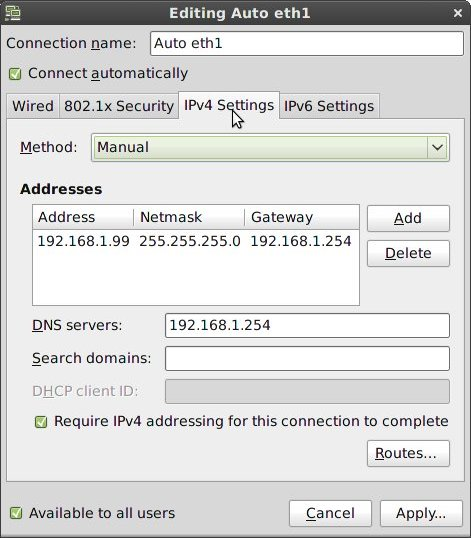
\includegraphics[width=\linewidth]{nm-ethernet.jpg}
			\caption*{Konfiguracija IP adrese}
		\end{minipage}
		\begin{minipage}{0.45\textwidth}
			\centering
			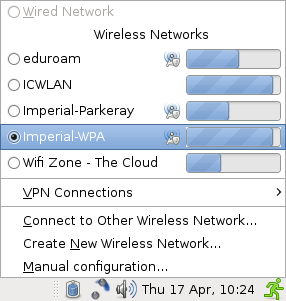
\includegraphics[width=0.8\linewidth]{nm-applet.png}
			\caption*{Odabir WLAN mreže}
		\end{minipage}
	\end{figure}
\end{frame}

\section{WLAN}
\begin{frame}
	\frametitle{WLAN}
	\begin{itemize}
		\item 802.11 a/b/g/n
	\end{itemize}
	Bežićna mreža je određena s
	\begin{itemize}
		\item SSID - naziv mreže
		\item BSSID - identifikator AP-a
		\item Sigurnosna razina
		\begin{itemize}
			\item Otvorena mreža
			\item WEP
			\item WPA - Personal i Enterprise
		\end{itemize}
	\end{itemize}
\end{frame}

\begin{frame}
	\frametitle{Podešavanje pristupa mreži}
	\framesubtitle{Pregled naredbi}
	\begin{table}[h]
		\rowcolors{1}{LightGray}{White}
		\begin{tabular}{l l}
			Pretraživanje mreža & \texttt{iwlist scan wl0}\\
			Odabir mreže (ESSID) & \texttt{iwconfig wl0 essid Ne\_kradi}\\
			Odabir mreže (SSID) & \texttt{iwconfig wl0 ap 00:11:22:33:44:55}\\
			& \texttt{iwconfig wl0 any}\\
			
			Spajanje na WEP mrežu & \texttt{iwconfig wlan0 essid}\\
			\hspace{1em} (hex ključ) & \hspace{1em} \texttt{Ne\_kradi key 0123456789}\\
			
			Spajanje na WEP mrežu & \texttt{iwconfig wlan0 essid}\\
			\hspace{1em} (string ključ) & \hspace{1em} \texttt{Ne\_kradi key s:password}
			
		\end{tabular}
	\end{table}
	
	\begin{itemize}
		\item Nakon spajanja na bežičnu mrežu slijedi uobičajena IP konfiguracija
		\item Za WPA mreže koristi se \texttt{wpa\_supplicant}
	\end{itemize}
\end{frame}

\begin{frame}[fragile]
	\frametitle{WLAN}
	\framesubtitle{wpa\_supplicant}
	\begin{itemize}
		\item Konfiguracija kroz \texttt{wpa\_cli} ili izravno \texttt{/etc/wpa\_supplicant.conf}
	\end{itemize}
	{\tiny \begin{verbatim}
$ wpa_passphrase MYSSID passphrase
network={
    ssid="MYSSID"
    #psk="passphrase"
    psk=59e0d07fa4c7741797a4e394f38a5c321e3bed51d54ad5fcbd3f84bc7415d73d
}
	\end{verbatim}
	\begin{block}{/etc/wpa\_supplicant/eduroam.conf}
	\begin{verbatim}
network={
   ssid="eduroam"
   proto=WPA2 WPA
   key_mgmt=WPA-EAP
   pairwise=CCMP TKIP
   group=CCMP TKIP
   ca_cert="<path_to_cert>/eduroam_fer.hr_CA.pem"
   subject_match="freeradius.fer.hr"
   identity="<USER>"
   eap=TTLS
   password="<PASSWORD>"
   phase2="auth=PAP"
}
	\end{verbatim}
	\end{block}}
\end{frame}

\section*{}
\begin{frame}
	\frametitle{Literatura}
	\footnotesize
	\url{https://wiki.debian.org/NetworkConfiguration}\\
	\url{https://wiki.archlinux.org/index.php/Network_configuration}
	\vfill
	\url{https://wiki.archlinux.org/index.php/iptables}\\
	\url{https://wiki.archlinux.org/index.php/Simple_stateful_firewall}
	\vfill
	\url{https://wiki.archlinux.org/index.php/Wireless_network_configuration}\\
	\url{https://wiki.archlinux.org/index.php/WPA_supplicant}
	\vfill
\end{frame}

\end{document}
